\chapter{Implmentation Plan}
The implementation plan of this work can be divided into two parts, FYP1 and FYP2. The tasks are then spreaded out into the two parts. Both gantt charts indicate the tasks and the time frame for each task. The gantt chart for FYP1 is shown in Figure 5.1 and the gantt chart for FYP2 is shown in Figure 5.2.

\begin{figure}[H]
  \centering
  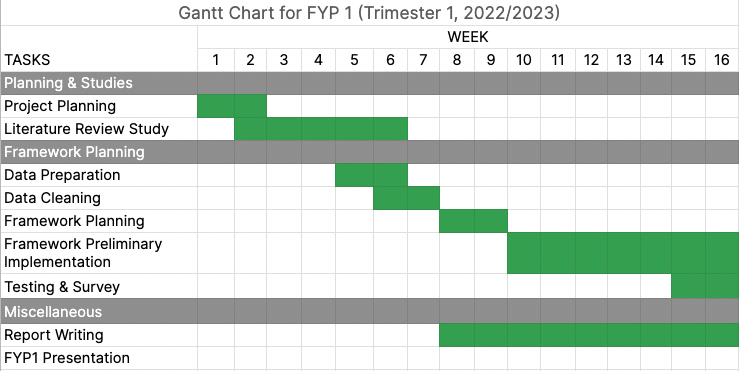
\includegraphics[scale=0.60]{assets/gc-1.png}
  \caption{Gantt Chart for FYP1}
  \label{fig:gc-1}
\end{figure}

\begin{figure}[H]
  \centering
  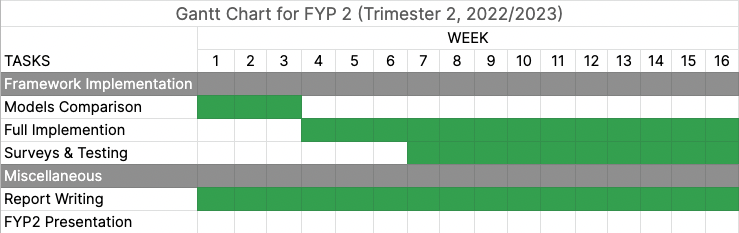
\includegraphics[scale=0.60]{assets/gc-2.png}
  \caption{Gantt Chart for FYP2}
  \label{fig:gc-2}
\end{figure}


\noindent The colored architecture framework also indicates the part of the framework that is being developed in FYP1 or FYP2. The architecture framework is shown in \ref{framework}.

\section{Project Target}
A good amount of research, planning and implementation was done in the FYP 1 phase, the solution A architecture was built and tested. The experiment indicates that there are improvements to be made in order to achieve excellency. Consequently, the FYP 2 phase will be focused on improving the solution A architecture and also implementing the solution B architecture. In addition, Deep learning models should be considered and compared with the current architecture to determine if deep learning models are better. At last, more data sources are also expected to be added to the framework to fully test it's capabilities.

\section{Web Application and Framework Hosting}
A web application written in the "React" framework will be developed to allow users to interact with the framework. While the framework itself will be hosted as an FAST API server. Both the web application and the framework will be hosted on the cloud platforms, Vercel and AWS respectively to allow public access to the solution.